\chapter{Research}

\label{ch:background}

\section{Introduction}

The main focus of the project is to provide new and experienced mobile developers with three deliverables. The deliverables will bring something new to the table, a new way of developing applications. These deliverables are as follows:

\begin{itemize}
  \item Mobile Back-end as a Service
  \item Mobile framework (SDK)
  \item Dashboard
\end{itemize}

This chapter will not only cover the background research required for the deliverables, but also research from mobile developers and general mobile users. It will also cover the technologies required along with the current similar solutions.

\section{Background}

\subsection{Project deliverables}

\subsubsection{Mobile Back-end as a Service}

BaaS is an approach for providing mobile app developers a way to connect their application to back-end cloud storage and processing while also providing common features such as user management, push notifications, storage, and other  features that mobile users demand from their apps these days. The objective of any developer is to get their product finished and publish as quickly as possible. By providing a MBaaS to developers, it reduces time and resources needed to develop an app. As a research paper from Kinvey \cite{kinveywebsite} states these points regarding what BaaS delivers:

\begin{itemize}
  \item Efficiency Gains
    - Reducing overhead in all aspects of mobile app development, increasing efficiency at all stages of development
  \item Faster Times to Market
    - Reducing the obstacles to take a mobile app from idea to production and overhead with operations once in production
  \item App Delivery With Fewer Resources
    - BaaS supports development with fewer developers and supporting data and IT resources
  \item Optimize for Mobile and Tablets
    - BaaS providers have put a lot of time and resources into optimization of data and network for mobile apps, and reduce fragmentation problems across multiple platforms and devices.
  \item Secure and Scalable Infrastructure
    -  BaaS provides a bundled infrastructure that deals with scalability, security, performance and other operational headaches, leaving developers to do what they do best
  \item Stack of Common API resources 
    - BaaS brings common and essential 3rd party API resources into a single stack, preventing developers from having to go gather them separately
\end{itemize}

After reviewing why developers should use a MBaaS, the research paper goes on to discuss a pattern of building blocks being to emerge. These are the basic services that any MBaaS provider should be offering.

\begin{itemize}
  \item User Management
    - It all starts with a user, the ability for users to sign up and log in.
  \item Storage
    - a central location for all app data to be stored to connect all users together.
  \item Rest API
    - the link between the back-end services and client applications.
  \item Communication
    - feature such as push notifications to keep users connected live with other users.
\end{itemize}

In the technologies section will go into what web-server will be used along with programming language required. 

\subsubsection{Mobile framework}

Mobile frameworks helps with dealing with complex project such as integrating the MBaaS in apps. This is accomplish by using a dependency manager, which is a tool that manages all of the libraries in a meaningful and logical manner. By dependencies, its the libraries to make the application work with the MBaaS. There are a few of iOS dependency managers which can be used which will discussed in the technologies section.

\subsubsection{Dashboard}

\subsection{Mobile developers}

The key part of this project is to research from experienced developers, asking them in person and in forums. I have put up multiple questions in different forums regarding the functionality required for mobile Baas; What advantages and disadvantages do you find with current third party mobile back-end as a services?, What features do you want to be included in these services that you do not see at the moment? and Where do you see the future of third party services going, are they required or should mobile developers implement their own back-end? I have not been quite successful with these forums questions as most questions have to be problem specific but I have had some feedback.

I met with Trust5 \cite{trust5} and Tapadoo \cite{tapadoo}, two mobile software developing companies based in Dublin, Ireland to discuss my project proposal. The general feedback was positive, seeing the potential and powerful tool it could be. I had a working prototype iPad app  to demonstrate the remote configuration service as part of my project which updates a client mobile app interface which I will explain later. See appendix for the case study of each company.

\subsection{Mobile users}

Surveys were created to help get mobile users feedback using apps. The reason for this to be part for the research is that they are the end-user. They are the ones we want to keep happy, keep using our apps. The survey contained a number of questions which along with the results are as follows:

\subsubsection{1. Would you delete an app if it crashes?}

\begin{figure}[!h]
    \centering
    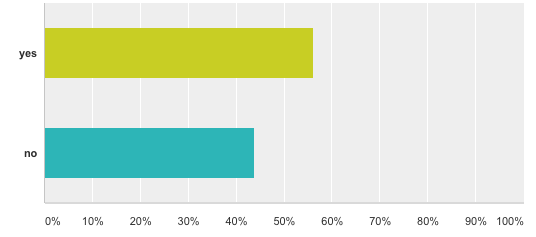
\includegraphics[width=100mm]{images/survey/crashes}
    \label{fig:label}
\end{figure}

\subsubsection{2. If you had a choice between two of the same type apps, Do you choose based on?}

\begin{figure}[!h]
    \centering
    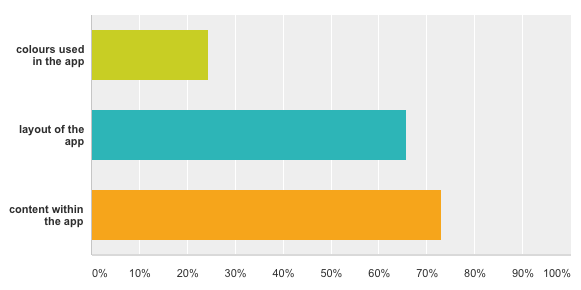
\includegraphics[width=100mm]{images/survey/choose}
    \label{fig:label}
\end{figure}

\subsubsection{3. How often do you like app updates?}

\begin{figure}[!h]
    \centering
    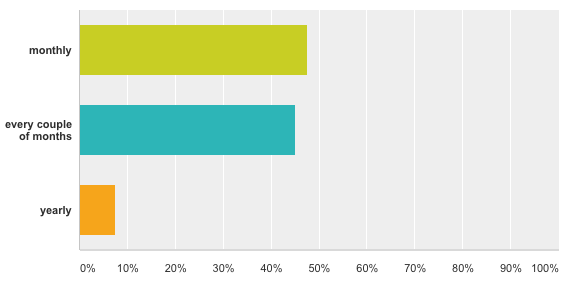
\includegraphics[width=100mm]{images/survey/time}
    \label{fig:label}
\end{figure}


\subsubsection{4. Would you prefer the user interface to be kept up to date and fresh more often?}

\begin{figure}[!h]
    \centering
    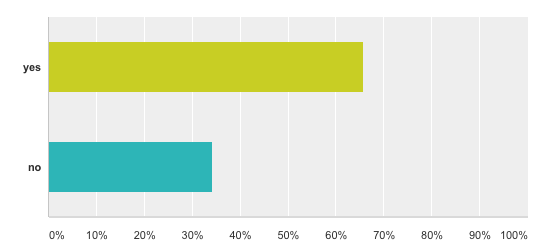
\includegraphics[width=100mm]{images/survey/updates}
    \label{fig:label}
\end{figure}

\subsubsection{5. Would you prefer being given the option for language choice (eg. English)?}

\begin{figure}[!h]
    \centering
    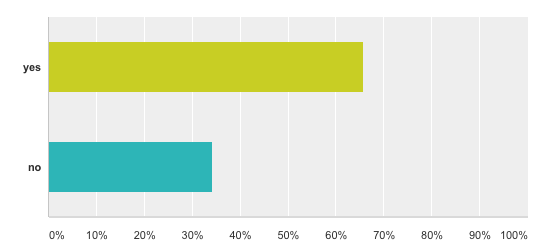
\includegraphics[width=100mm]{images/survey/language}
    \label{fig:label}
\end{figure}


\subsubsection{6. Do you mind apps collecting analytics in the background to help improve the app ? (not personal information)}

\begin{figure}[!h]
    \centering
    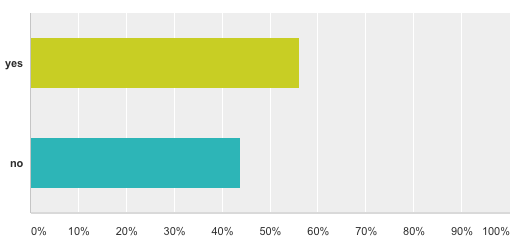
\includegraphics[width=100mm]{images/survey/analytics}
    \label{fig:label}
\end{figure}


The above survey gives an understanding on what users feel when using apps, also some insight into what they want to have more often. By asking a users these questions, it has given a meaningful reason to implement one of the key features to be implemented in the project. A feature that enables developers to keep the app updated quicker for users to feel like they are not forgotten, to give the app a new look and feel. But also a quick way to stop the user from deleting the app because it crashes. This will be further discussed in the design chapter.


% --------------------------------------------%
% Technologies researched
% --------------------------------------------%

\section{Technologies}

\subsection{Programming Languages}

\subsubsection{Objective-C}
Objective-C \cite{objectiveC} is an object-oriented programming language developed in early 1980s.  It was used to develop on NeXT OS which later became OSX and iOS.  Objective-C is a super set of the  C programming language meaning that it is possible to compile any C program with an Objective-C compiler. 

\subsubsection{Swift}
Swift \cite{swift} is Apple’s latest open-source programming language used mainly for developing on iOS, macOS, watchOS and tvOS applications.  Swift it an alternative to the Objective-C language, but is sometimes referred to Objective-C without the C. In contrast to Objective-C, it does not expose pointers to refer to object instances. Swift does retain Objective-C concepts including protocols, closures and enums. It was designed to make writing and maintaining programs easier for developers.

\subsubsection{Python}
Python \cite{python} is a high level programming language. It is designed to allow programmers to express concepts in fewer lines of codes than possible such as Java or C++. It is the perfect language to write programs on both a small and large scale. It supports object-oriented (OOP) and functional programming. Python was first created in the late 1980s by Guido van Rossum as a successor to the ABC language.

\subsection{Web Frameworks}

\subsubsection{Perfect (Server-side swift)}
Perfect \cite{perfect} is a web server and toolkit for developers using the swift programming language to build applications and other REST services. It can be deployed on macOS and Linux server.

\subsubsection{Kitura (Server-side swift)}
Kitura \cite{kitura} is a web server and web framework for Swift 3 developed by IBM. It is similar to Perfect, using core Swift technologies.

\subsubsection{Django}
Django \cite{django} is an open-source  high level Python web framework which follows the Model-View-Controller (MVC) pattern.  It consists of an object-relational mapper (ORM) that maps models (M)  defined as Python classes to a relational database, a system for processing  HTTP request to a web view (V).  It focuses on rapid development and the principle of  “don’t repeat yourself” and scalable. It was born in 2009 by few web developers and began to use Python to build applications. Django looks after authenticating the user when signing up, signing in and signing out. Python is used throughout the development even for setting files and creating models. Popular site such as Pinterest, Instagram and Bitbucket use Django for their web framework.

\subsubsection{Flask}
Flask \cite{flask} is a micro web framework written in Python and initially released in 2010. Applications such as Pinterest and LinkedIn use this framework. It is called micro framework as it does not require any dependencies to run, as well as that it does not have extra layers such as database but supports extensions that can be added to create extra features. Flask is popular among Python enthusiasts and was the most popular Python web framework on Github.

\subsubsection{Node.JS}
Node.JS \cite{node} is an open-source cross platform environment originally released in 2009. It is used to create a variety of tools and applications such as GoDaddy, Groupon and Paypal.  It is driven by events such as when a consumer purchases an item. Node.js has been optimized for web applications with many input/output operations, as well as real-time communication.

\subsection{Dependency Managers}

\subsubsection{CocoaPods}

CocoaPods \cite{pods} is the de facto standard of package management for iOS. It has the largest community and is officially supported by almost every open-sourced iOS library. It contains over twenty eight thousand libraries which are used in over 1.8 million apps.

\subsubsection{Carthage}

Carthage \cite{carthage} is intended to be the simplest way of add frameworks to apps. It was the first dependency manager for macOS and iOS, created by group of developers from Github. It was also the first dependency manager to work with Swift. It exclusively uses dynamic frameworks instead of static libraries, this is the only way to distribute Swift binaries that are supported by iOS 8 and up.

\subsection{Databases}

\subsubsection{MySQL}
MySQL \cite{sql} is an open-source relational database management system (RDBMS) initially released in 1995. Previously owned by a swedish company MySQL AB and now owned by Oracle Corporation. MySQL works on many system such as macOS, Windows, Linux, FreeBSD so making it a common choice and reviews are positive.

\subsubsection{MongoDB}
MongoDB \cite{mongoDB} is also a free and open-source database type program, but is a document-oriented. Classified as a not-only SQL (NoSQL) which uses JSON like documents to store objects. Features includes indexing, replication, load balancing and the list goes on. The main difference of MongoDB is that it is not a relational database. Objects that are related somewhat together are stored together in one file, improving retrieval of data.

\subsubsection{PostgreSQL}
PostgreSQL \cite{postgreSQL} is an object-relational database with additional object features. It differs itself support for highly required and integral object-oriented and relational database functionality, such as complete support for reliable transactions. It also free and open-sourced, yet very powerful with the capabilities of storing procedures.

\subsection{Web servers}

\subsubsection{Apache}
Apache \cite{apache} was created by Robert McCool in 1995 and has been furthered developed by Apache Software Foundation since 1999. The Apache web server has been the most popular server since 1996. Administrators choose this for its flexibility, power and widespread support. Apache creates processes and threads to handle additional connections. The admin can configure the server to control the maximum number of allowable processes, which is depending on the amount of physical memory. Each connects gets it own new thread which handles on user request.

\subsubsection{Nginx}
Ngnix \cite{nginx} was developed by Igor Sysoev in 2002, which answered to the problem that web-servers began handling ten thousands concurrent connection. It was initially released in 2004. Nginx has grown due to its light-weight resource utilization and its ability to scale. Nginx works different to Apache, in that it does not create new processes for each web request, instead the admin configures how many worker processes to create. The rule of thumb is that one work process for each CPU. Each worker can handle thousands of requests.

\subsection{Cloud Computer Services (IAAS)}

\subsubsection{Amazon Elastic Computer Cloud (EC2)}
%reword
EC2 " is a web service that provides secure, re-sizable compute capacity in the cloud. It is designed to make web-scale cloud computing easier for developers." \cite{ec2} Amazon EC2 is widely used by companies such as Netflix, AirBnB and Expedia. It can be used to launch as many or as few virtual servers as needed, that can be configured to suit your needs.

\subsubsection{DigitalOcean server}

DigitalOcean \cite{digital} is an American cloud infrastructure provider. It provides developers cloud services that help to deploy and scale applications that run simultaneously on multiple computers. As of December 2015, DigitalOcean was the second largest hosting company in the world in terms of web-facing computers. Within a few steps, you can have web-server up and running. The perfect choice for this project, that can set-up a Ubuntu 16.04 server in a matter of minutes. 

\newpage
\subsection{Evaluation}

% \usepackage[table,xcdraw]{xcolor}
% If you use beamer only pass "xcolor=table" option, i.e. \documentclass[xcolor=table]{beamer}
\begin{table}[!h]
\centering
\caption{Findings}
\label{my-label}
\begin{tabular}{|l|l|l|}
\hline
\cellcolor{green!20}Technology & \cellcolor{green!20}Version  & \cellcolor{green!20}Area \\ \hline
Swift      & 3.0.1      & Client Framework/Back-end Language \\ \hline
Linux      & 16.0.4 X64 & Server OS                          \\ \hline
MongoDB    & 3.2.11     & Cloud Storage                      \\ \hline
Flask      & 0.1.1      & Test Web Framework                 \\ \hline
CocoaPods  & N/A        & Dependency Manager                 \\ \hline
DigitalOcean    & N/A     & Cloud Service               \\ \hline
Nginx            & 1.10.3       & Web server               \\ \hline
Perfect            & 2.0      & Web Framework               \\ \hline
\end{tabular}
\end{table}

\subsubsection{Programming Language}

Chosen technologies as a result from the research for client side application is Swift for both the framework and dashboard app. I decided to go with Swift for client side programming for few different reasons but one that stood out was a blog from 9To5Mac website \cite{webserver}. At the beginning of 2016 Swift took over Objective-C making it the 14th most popular programming language. Protocol Oriented Programming (POP) is an interesting concept mainly used in Swift. It is starting to become commonly used instead of Object Oriented Programming (OOP) because objects are “things” that encapsulate complexity. So an object does it in a certain way, but protocols can provide objects with doing it different ways. With POP, the interface being what the user interacts with it the main and only concern.

\subsubsection{Dependency Managers}

A-Coding blog review goes into the pros and cons of both CocoaPods and Carthage \cite{acodingwebsite}. CocoaPods has a large community behind it, so problems can be easily help and resolved. There are a large number of available libraries and are listed on their website: https://cocoapods.org. It has a centralised file that manages all libraries required for the app along with version. But because it is centralized, if it goes down you will be affected.

Carthage is not centralised, each dependency is fetched from their original repositories. It can be very slow managing all dependencies, especially if the app requires a large number of them. Some find CocoaPods invasive as it modifies the Xcode project by building its own workspace. However Carthage does not, it is up to the developer to add the required libraries into their project.

Due to extensive help from the community, and the project is all about helping the developer with reducing the amount of development, the project will be using the CocoaPods dependency manager for the MBaaS framework.


\subsubsection{Web Framework}

The project is aiming to be open-source, so that developers can contribute towards it. So without needing to learn a different language like Python for Django, the choice is a web-server using Swift language. As swift is becoming more popular and has become open-source, it is reasonable conclusion that the near future will include more back-end servers written in swift.

Now the web framework choose it based on Swift programing language, the choice is between Perfect and Kitura. A bench-marks was conducted by Ryan Collins, a web developer. He posted a blog about the outcome \cite{benchmark} which clearly shows that not only is both Perfect and Kitura faster than Node.JS but that Perfect is the leader. The blog goes into detail of the test that was run, the server setup and the number of requests made.

\begin{figure}[!h]
    \caption{Benchmark}
    \centering
    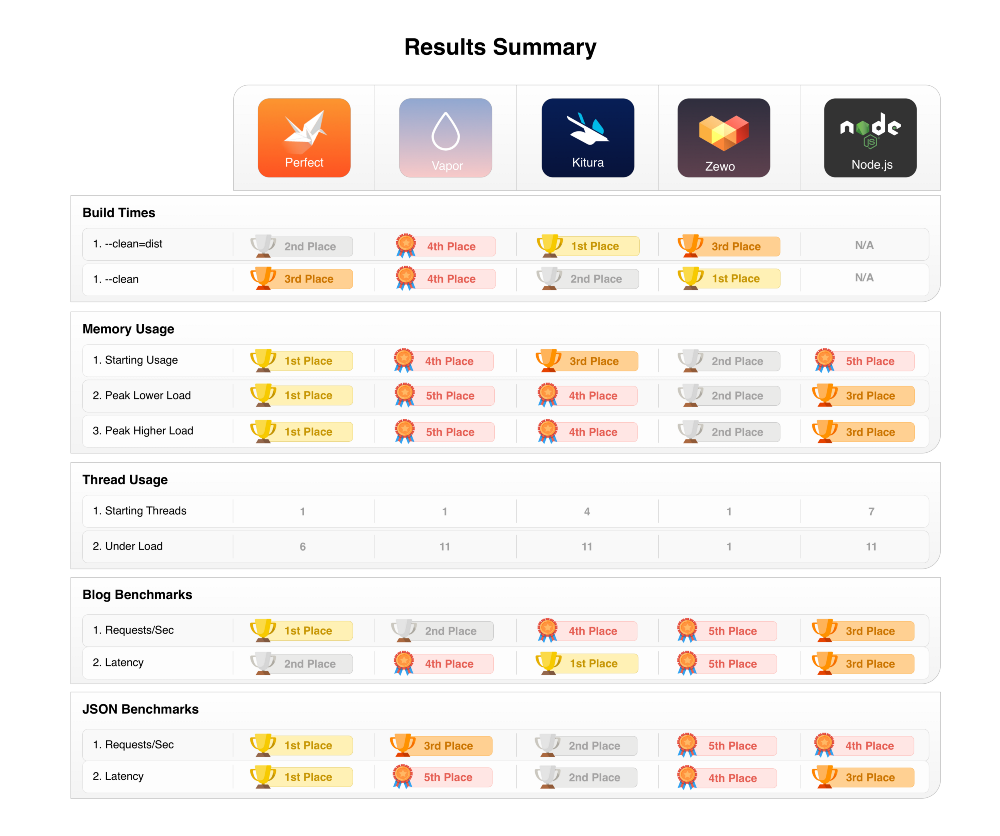
\includegraphics[width=75mm]{images/benchmarks}
    \label{fig:label}
\end{figure}

The result as stated in the blog, is that Swift is more capable of taking on the established server side frameworks. So regarding what Swift web framework to use, the decision is Perfect with over 10,000 stars on the Github repository. \cite{github1} 

\subsubsection{Database}
The database choice is MongoDB which is a NoSQL. It provides a dynamic way of storing data where object properties name and type are unknown until run time. This allows the system to be implemented with different types of data being sent and gives the developers less stress without having to worry about what models need to be created at design time. From the article “When to use MongoDB rather than MySQL” \cite{database} the reasons for choosing MongoDB is when:
\begin{itemize}
  \item Expect a high load amount of data
  \item Need to grow big 
  \item Do not have a database admin
\end{itemize}
The above 3 reasons are compelling enough to choose MongoDB because when designing a back-end as a service for applications of any type, then freedom and flexibility are key. Another valid reason is when you do not know the database structure and when providing a service to developers to give them tools to create any database structure is another strong reason to go with MongoDB. 

\subsubsection{Cloud Computer Services (IAAS)}
Digital Ocean

\subsection{Web servers}
Nginx has be decided for the project.

\subsection{Extra tools required}

\subsubsection{Xcode}

Xcode is an integrated development environment (IDE) containing a suite of software development tools developed by Apple for developing software for macOS, iOS and tvOS. First released in 2003, the latest version 8 is free download via Mac App Store. It supports source code for programming languages C, C++, Objective-C and Swift etc. 

\subsubsection{Swift Playgrounds}

Swift playground also know as just playground is an interactive work environment that allows you see the values in the sidebar for the written code. As and when you make changes to your code the sidebar reflects the changed result. It was introduced in Xcode 6 and enhanced in Xcode 7 that make learning Swift and experimenting much easier. Instead of having to create a app just to run and test some Swift code, a smaller playground can be made to view the outcome of each test piece. 

\subsubsection{APNs Auth key}

The Apple Push Notifications (APNs) involves generating an authentication key, that will sit on the server and will send notifications to one or more devices. Until recently, the generating of the authentication key consisted of painful steps. These include filling out a Certificate Signing Request in Keychain Access, then uploading it to your developer account. After which downloading a signed certificate, to which converting to .pem format. Also certificate would then expire, so the steps would need to be done again every year.

Now Apple has greatly improved this service, which involves the creation of one key of type .p8, which does not expire. The downloaded file, can then without converting be upload to the server to be used. Apple also gives three text keys that are used in authenticating the APNs and send the notifications. These include; APNs Auth key, Team ID and the App ID.

\subsubsection{Github}

Github \cite{github} is a web-based version control repository. It provides code sharing, publishing, deployment and much more. The developer can create as many private or public repositories as required. Github provides developers with tools to backup, version control and create branches to separate out builds.

\subsubsection{Perfect Assistant}
"This macOS companion application is a set of convenience tools designed to help Server Side Swift developers start, manage, compile, test, and prepare for deployment more easily. From those expanding into backend Swift development for the first time to seasoned senior engineers working on enterprise level projects, the Perfect Assistant will facilitate your work." \cite{perfectAssist} It is used to help include all the required packages required to build the project, and includes tools to deploy to amazon web-server and docker.


% --------------------------------------------%
% Similar Technologies researched
% --------------------------------------------%
% \newpage

\section{Similar Technologies}

\subsection{Overview}

\begin{table}[h]
\centering
\caption{Alternative Solutions}
\label{fig:overview}
\begin{tabular}{|l|l|l|l|l|}
\hline
\cellcolor{green!20}Service &\cellcolor{green!20}Parse &\cellcolor{green!20}Firebase &\cellcolor{green!20}BassBox &\cellcolor{green!20}Amazon \\ \hline
Notifications               & Yes                      & Yes                         & Yes                        & Yes\\ \hline
Database                    & Yes                      & Yes                         & Yes                        & Yes\\ \hline
Analytics                   & Yes                      & Yes                         & No                         & Yes\\ \hline
self hosted                 & Yes                      & No                          & Yes                        & No \\ \hline
Remote configuration        & No                       & Yes                         & No                         & No \\ \hline
Backup                      & No                       & No                          & No                         & No \\ \hline
User Sign-Up                & Yes                      & Yes                         & Yes                        & Yes\\ \hline
A/B Testing                 & No                       & Yes                         & No                         & Yes\\ \hline
\end{tabular}
\end{table}


\subsection{List}

\subsubsection{Parse}

\begin{figure}[!h]
    \caption{Parse}
    \centering
    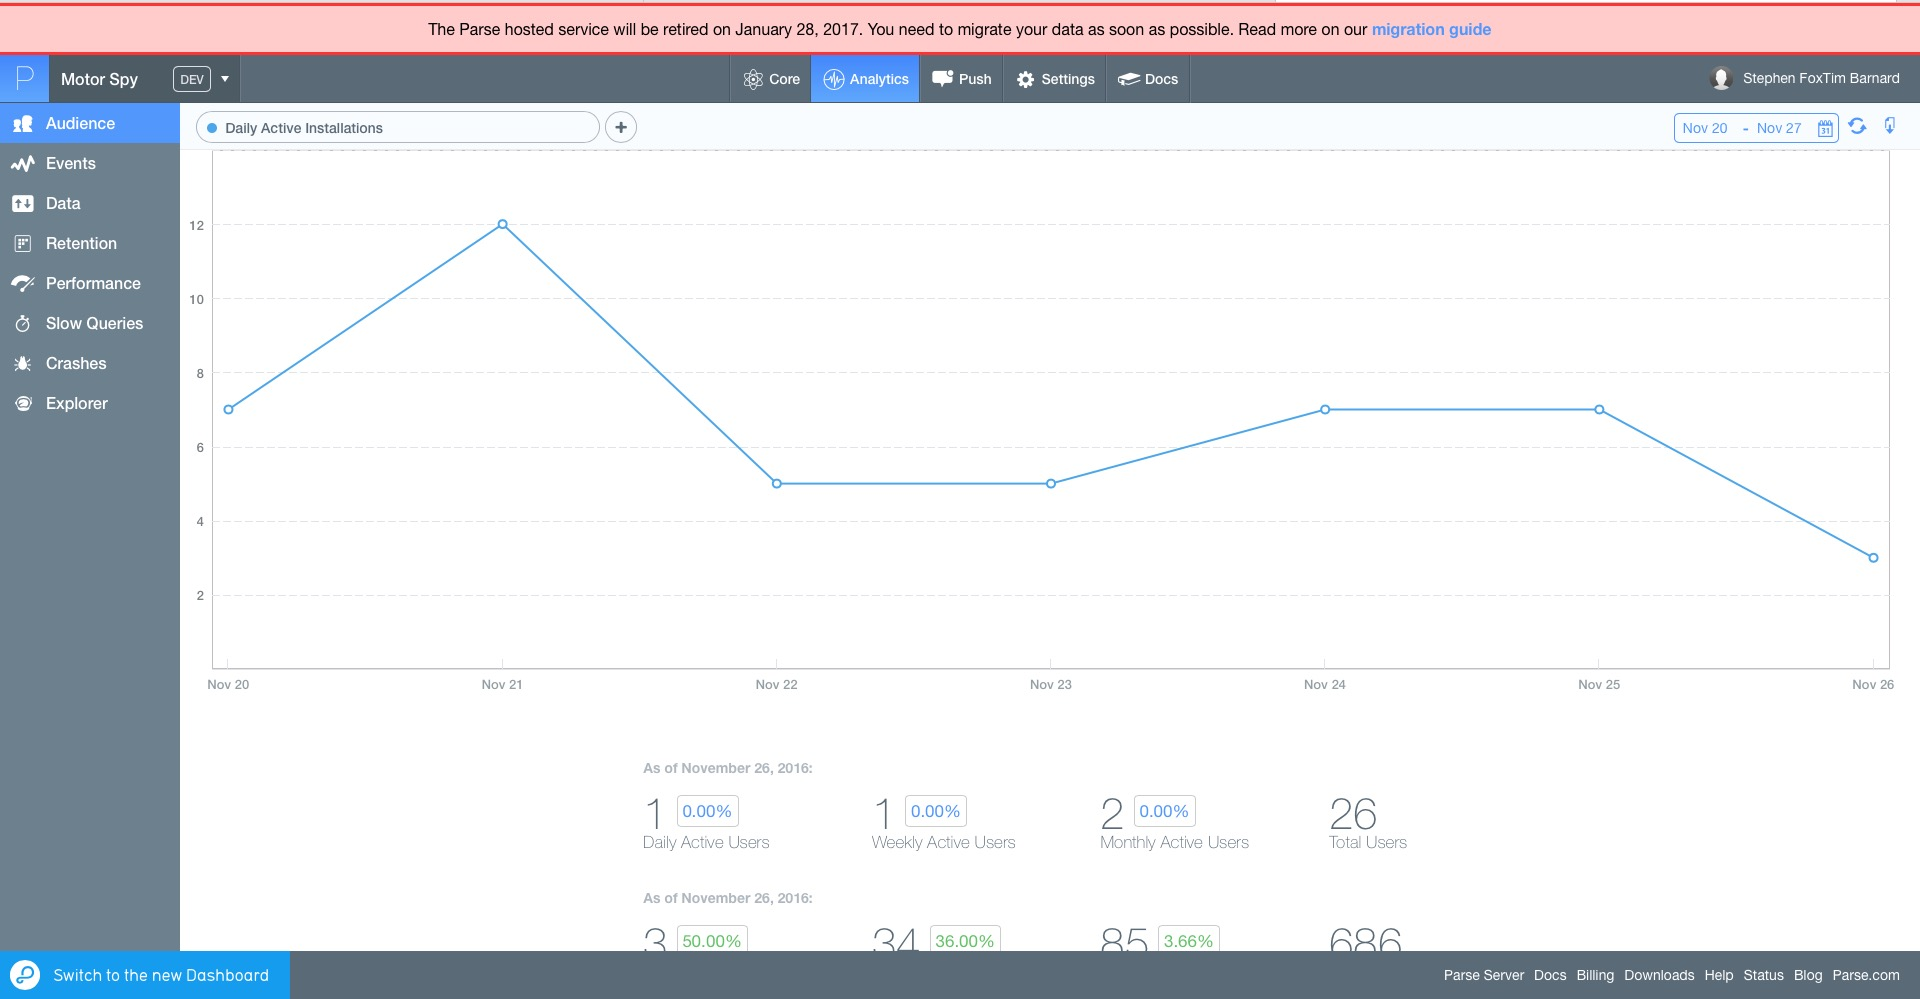
\includegraphics[width=100mm]{images/parse}
    \label{fig:parse}
\end{figure}

Parse \cite{parse} was founded in 2011 by Tikhon Bernstam, Ilya Sakhar, James Yu and Kevin Lacker former Google and Combinator employees. The project kick-started when it raised 5.5 billion dollars in funding in late 2011 and by 2012 over 20,000 mobile developers were using the service. Facebook in 2013 acquired the company for 85 million dollars and continued to grow. By 2014 500,000 apps were using the service, but sadly Facebook in 2016 announced that they are closing down the service in January 2017. They do provide tools and tutorials on how to migrate to your own hosted service. The service when operational was widely used by developers and Fig \ref{fig:parse} shows the main dashboard page. One of the developers mentioned in the interview that his company Tapadoo used to use Parse before they announced the closure of the service.

\subsubsection{Firebase}

\begin{figure}[!h]
    \caption{Firebase}
    \centering
    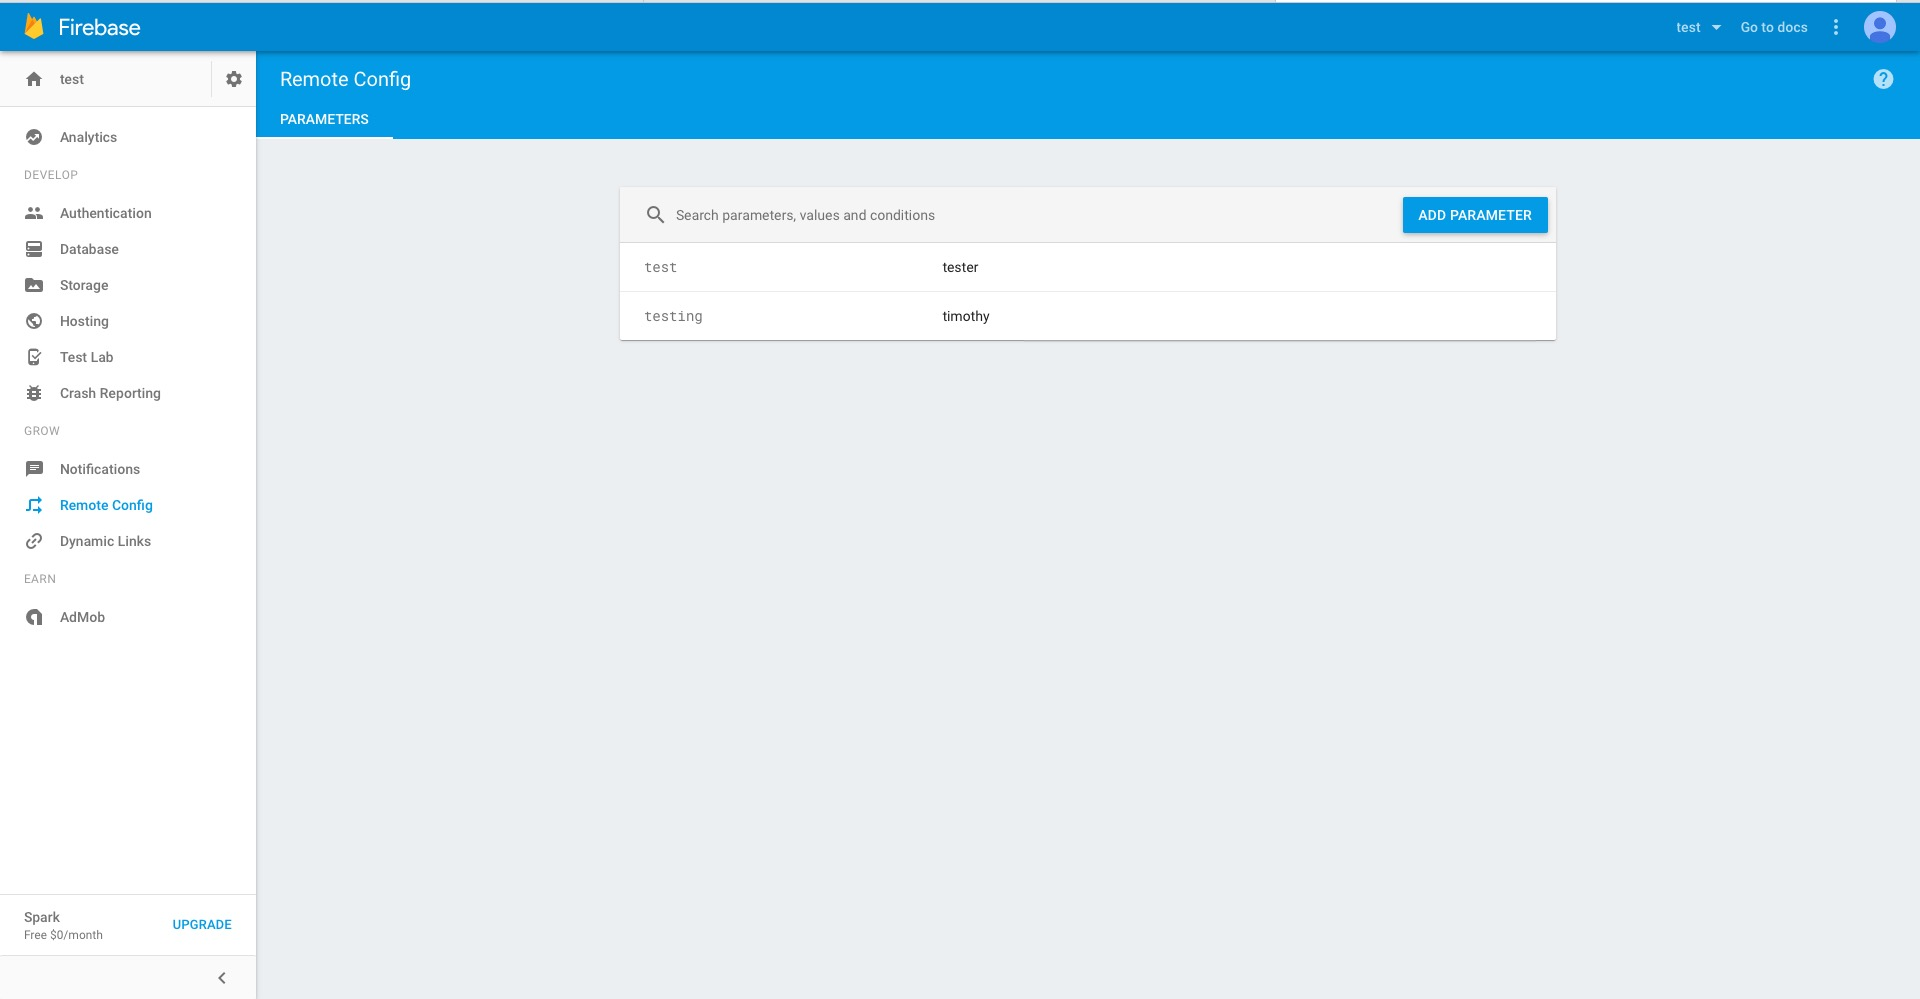
\includegraphics[width=100mm]{images/firebase}
    \label{fig:firebase}
\end{figure}

Firebase \cite{firebase}  evolved from Envolve, a start-up founded by Tamplin and Lee in 2011. They provided a service that enabled developers to integrate on-line chat into their web site but found after a while that the service was being used to pass application data that was not chat messages in real time. So the team decided to separate the chat system and real time architecture that powered it. This lead to the founding of Firebase, a separate company. 
It raised funding in 2013 and in 2014 Google acquired the company for an undisclosed amount. The company provides a list of services as shown in Table \ref{fig:overview} for free for limited amount of users and storage of 5GB, but as you increased the storage and users using your application then so does the price. If we way in more storage, real-time database space then the price per month is around 200 dollars \cite{firebase2}. The dashboard for managing your project is shown in Fig \ref{fig:firebase}, the current page is remote configuration service.

\subsubsection{BaasBox}

\begin{figure}[!h]
    \caption{BaasBox}
    \centering
    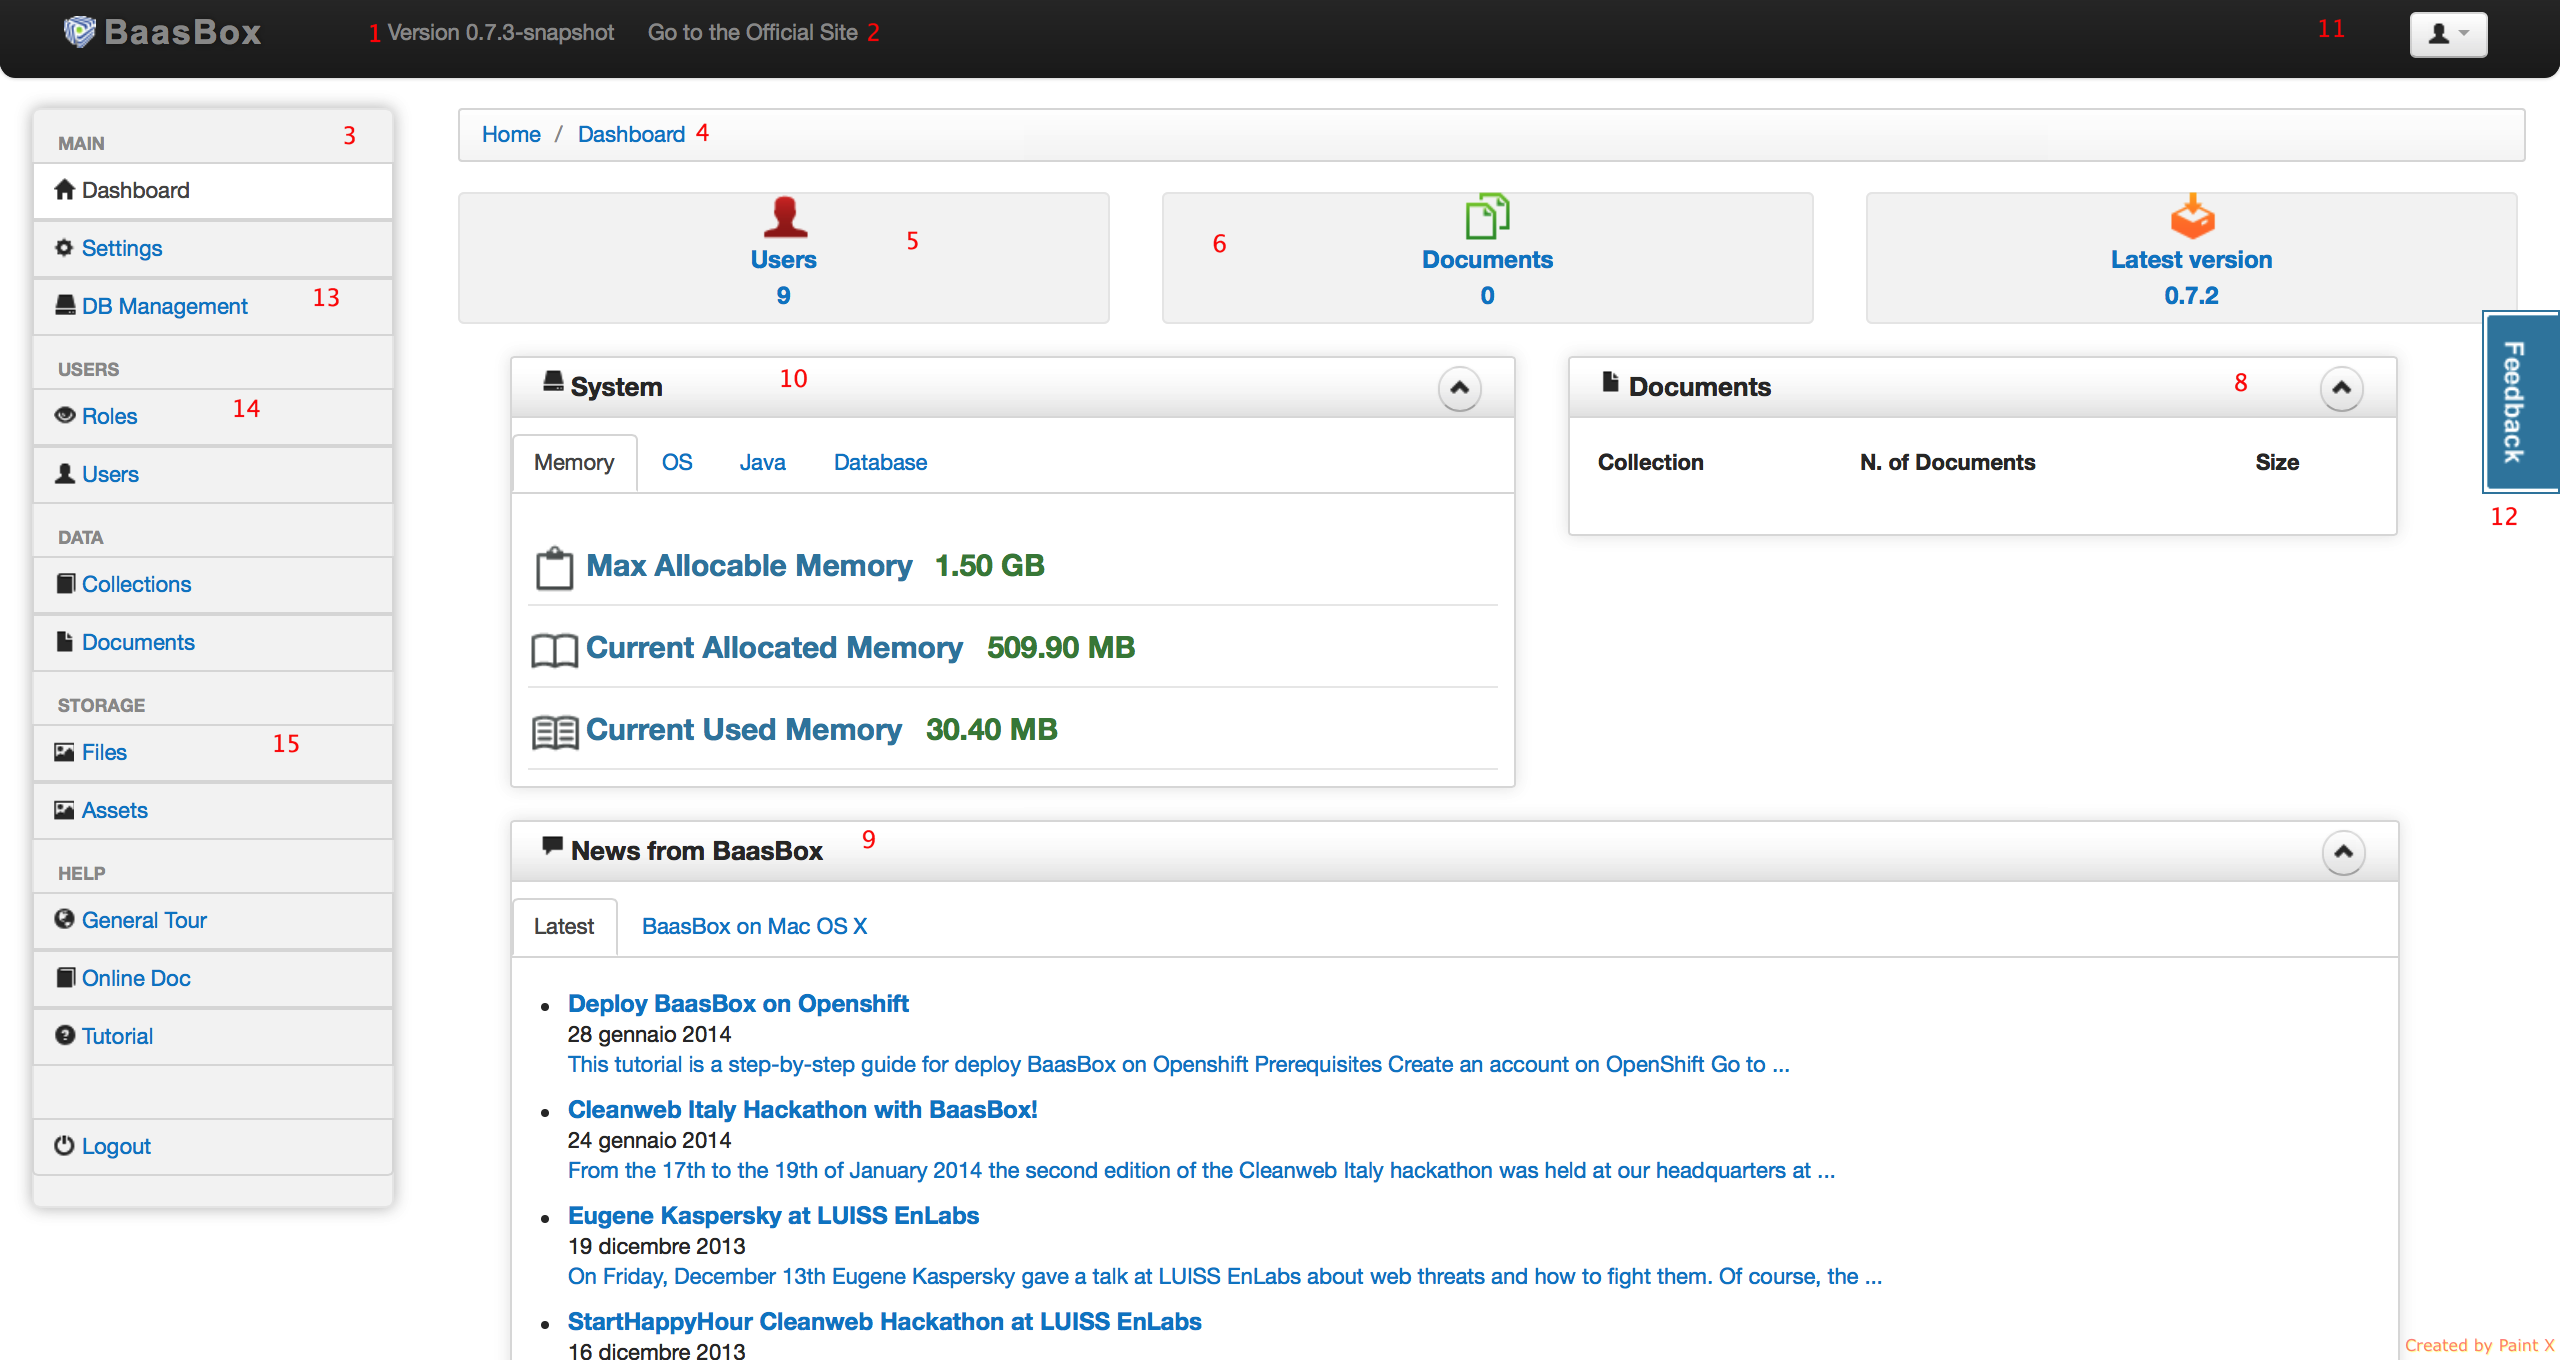
\includegraphics[width=100mm]{images/baasbox}
    \label{fig:baasbox}
\end{figure}

BaasBox \cite{baasBox} is an open sourced project founded in 2013, it is an application that acts a database and application server combined. It provides developers with an API as a back-end to store data for their mobile and web applications. It is the first back-end as a service to be open source and free to download. BaasBox also provides cloud services so instead of hosting the back-end on your own server. Fig \ref{fig:baasbox} shows the dashboard main page, on the left panel are a list of services they provide such as database.

\subsubsection{AWS}

\begin{figure}[!h]
    \caption{AWS}
    \centering
    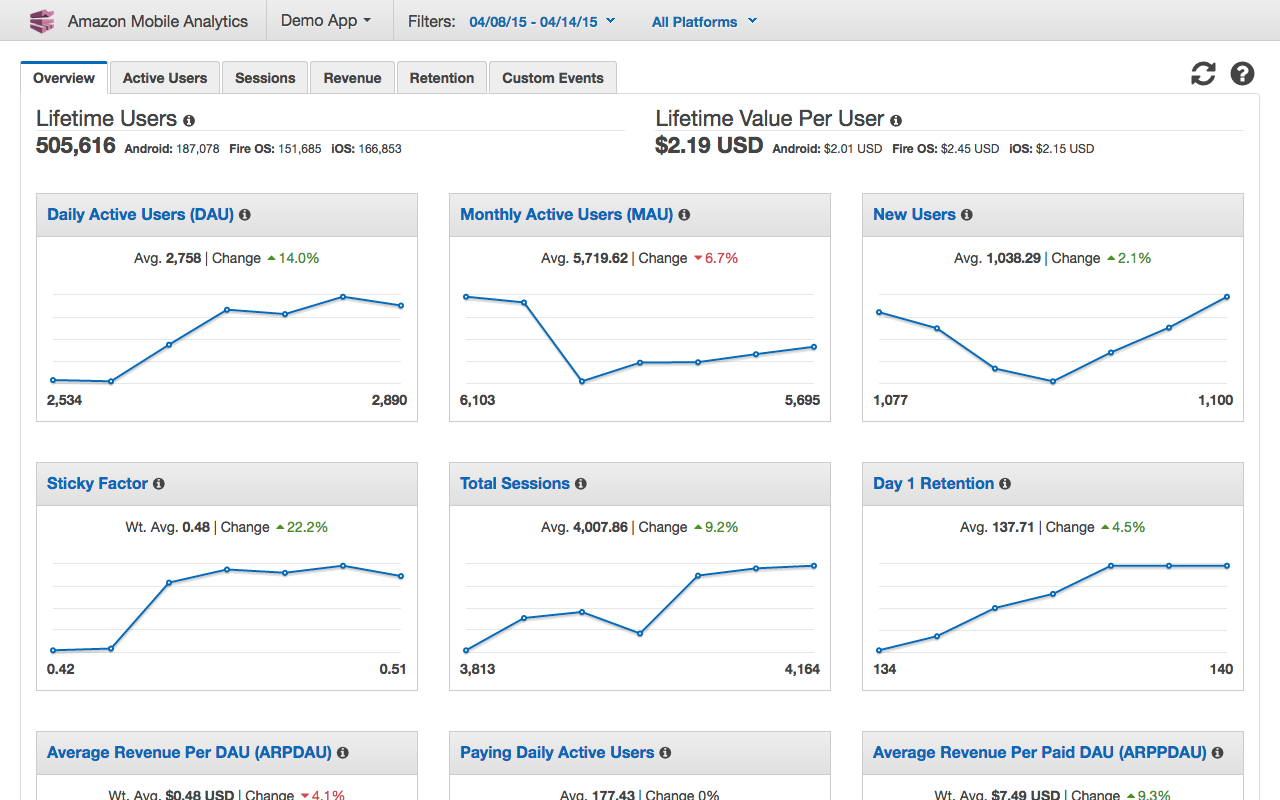
\includegraphics[width=100mm]{images/aws}
    \label{fig:aws}
\end{figure}

Amazon Web Services(AWS) \cite{aws} is a subsidiary of Amazon.com which offers a suite of cloud computing services launched in 2006.  By 2007 amazon claimed that more than 180,000 developers had signed up to use AWS Amazon Web Services. One of its services to AWS Mobile Services, a way to provide help to develop mobiles apps than can scale to hundreds of millions of users. Popular companies such as AirBnB and Netflix uses AWS mobile services to power their applications. Like other MBaaS providers, they do offer a limited 12 month free tier which includes 5GB of standard storage, 20,000 get requests and 2,000 put requests. Then outside of these limits the price does rise. The list of services they provide include analytics shown in Fig \ref{fig:aws}.


% --------------------------------------------%
% Requirements researched
% --------------------------------------------%
% \subsection{Requirements}

% After researching on similar technologies currently out their have lead me to the basic requirements. This include the following
% \begin{itemize}
%   \item Storage
%   \item Notifications 
%   \item Analytics
%   \item Sign up
% \end{itemize}

% Next came to part which is the reason why I wanted to do this project. A large challenge of a single developer without the money and resources for a design team, is struggling to think what end-users will like. This brought me to the next service requirement; A/B Testing. Also known as split testing is comparing two versions of a page to see which performs better.

\section{Human Computer Interaction}